\documentclass[11pt,a4paper]{report}
\usepackage[left=3cm,right=3cm,top=3cm,bottom=3cm]{geometry}
\usepackage[utf8]{inputenc}
\usepackage[francais]{babel}
\usepackage[T1]{fontenc}
\usepackage{graphicx}
\usepackage{blindtext}
\usepackage{listings}
\usepackage{amsmath}
\usepackage{amssymb}

\makeatletter
\renewcommand{\@chapapp}{Exercice}
\makeatother

%\setlength{\parindent}{0.7cm}
\setlength{\parskip}{\baselineskip}

\begin{document}

\begin{titlepage}

\centering

\includegraphics[scale=0.4]{SU.png}\par\vspace{1cm}
\vspace{1cm}
{\scshape\bfseries ARA\par}
\vspace{1.5cm}
{\huge\bfseries Projet Peersim\par}
\vspace{2cm}
{\Large\itshape Robin Blottiere-Mayo\par
	Pierre Oumeddour\par}
\vfill
{\Large Professeur : Jonathan Lejeune}
\vfill

% Bottom of the page
{\large \today\par}
\end{titlepage}

\pagenumbering{arabic}

\chapter{}

\section{Question 1 :}

L'algorithme de verrouillage utilisé dans la classe Application est un algorithme dérivé de celui de Naimi-Tréhel utilisant la notion de jeton.
%\linespread{0.5}

Ainsi tous les sites se partagent le même jeton et seul le site possédant le jeton peut entrer en section critique. Dans la classe Application, les constantes initial\_owner et nil servent à discriminer le site possédant le jeton des autres.
%\linespread{1.7}

Chaque noeud maintient sa propre liste de noeuds en attente de section critique (variable next) et son compteur global de sections critiques (variable global\_counter). Il possède également l'adresse du noeud dont il pense qu'il possède le jeton (variable last) ainsi que le nombre de sections critiques qu'il a lui-même effectuées (variable nb\_cs). Si un noeud veut une section critique, il envoie une demande pour avoir le jeton puis il se met en attente.
%\linespread{0.5}

Quand un noeud sort de section critique, il envoie le jeton au dernier noeud de la liste des noeuds demandant la section critique avec les informations qu'il possède du nombre de sections critiques réalisées et des noeuds en attente de section critique.
%\linespread{0.5}

Lorsqu'un noeud reçoit le jeton, il met à jour son compteur de sections critiques avec la valeur envoyée par le dernier noeud ayant été en section critique. Il compare également sa liste de noeuds en attente avec celle qu'il a reçue. Si des noeuds se trouvent dans les deux listes mais pas dans le même ordre, l'ordre envoyé par le dernier noeud en section critique est maintenu. Si des demandes sont absentes de la liste reçue, elles sont ajoutées en fin de liste.


\section{Question 2 :}

On considère trois états du jeton :
\begin{enumerate}
	\item Un noeud possède le jeton mais ne s’en sert pas (état tranquille).
	\item Un noeud possède le jeton et est en section critique (état utilisé).
	\item Le jeton est en transit (état enTransit).
\end{enumerate}

tranquille $\rightarrow$ utilisé : la section critique est demandée et personne ne requiert le jeton.\\
tranquille $\rightarrow$ enTransit : un noeud requiert le jeton.\\
utilisé $\rightarrow$ tranquille : la section critique se termine.\\
utilisé $\rightarrow$ enTransit : releaseCS(timeout) \& !next.isEmpty()\\
enTransit $\rightarrow$ utilisé : receive\_token()\\

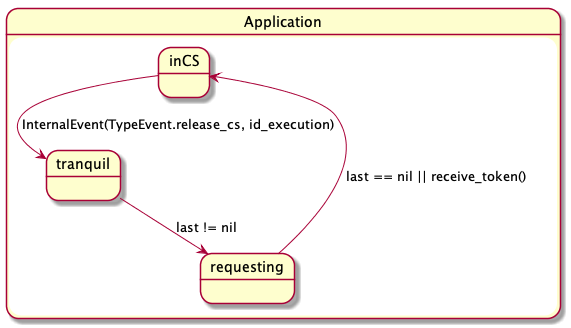
\includegraphics[scale=0.3]{../Diagrammes/exercice_1-question_2.png}


\section{Question 3 :}

$\alpha$ étant le temps moyen qu'un processus passe en section critique et $\beta$ le temps passé entre les sections critiques.

Le ratio $\rho$ = $\alpha$ / $\beta$ représente la charge du réseau.

Plus ce ratio est élevé plus le réseau est ralenti.

\section{Question 4 :}

\textbf{Messages applicatifs}:

Sur cette première courbe, on observe deux valeurs qui varient en fonction de la charge du réseau $\rho$. Il s'agit du nombre moyen de messages applicatifs par section critique. On différencie le nombre de messages requérents le jeton et le nombre de transmissions du jeton entre les noeuds.\\

On observe que plus $\rho$ augmente, plus le nombre de messages applicatif diminue. A la fin, il est quasiment de un message et un envoie de jeton par sections critiques. En effet, plus le temps passé en section critique est grand par rapport au temps d'attente plus les noeuds savent qui est celui possédant le jeton.\\

Cela s'explique par le fait qu'un noeud ayant fini sa section critique va s'endormir pour un temps qui sera court étant donné les paramètres de l'expériance qui incluent un temps de transmission et un temps de repot court entre les sections critiques. En se réveillant, le noeud enverra une requête de section critique au noeud dont il pense qu'il possède le jeton. Ce noeud aura en effet toujours le jeton en sa possession car il n'aura probablement pas eu le temps de terminer sa section critique. Ainsi, une seul requête aura suffi au noeud pour être repertorié comme demandant l'accès à la section critique. C'est pourquoi on observe quasiment un envoie de requête par section critique.\\

Cette explication est valable pour un temps d'expériance suffisament grand pour que les noeuds aient le temps de s'ordonner mutuellement.\\

\textbf{Temps passé dans l'état requesting}:

Sur cette courbe, on observe le temps moyen qu'un noeud passe dans l'état requesting en fonction de la charge du réseau.\\

On peut voir que lorsque que le temps $\beta$ passé entre les sections critiques est beaucoup plus grand que le temps $\alpha$ passé en section critique, le temps moyen par sections critique est très feible. Lorsque $\rho$ s'approche de un, le temps passé en section critique augmente très rapidement. Après cela, l'augementation redevient proche voir inférieur à un sur une échelle logarithmique.\\

Cette brusque augmentation peut s'expliquer par le fait qu'un temps $\alpha$ très court peut faire qu'à un certain moment, aucun des cinquante noeud du réseau ne requiert la section critique. Lorsque la charge du réseau sera suffisament grande pour qu'il y ait en permanance un noeud demandant l'accès à la section critique, le temps passé dans l'état requesting augmentra linéairement en fonction du temps ou le jeton est utilisé par un processus en section critique.\\

\textbf{Utilisation du jeton}:

Sur cette troisième courbe, on observe le temps que le jeton passe dans chacun des états décrits à la question 2 en fonction de la charge du réseau. L'expériance s'appuyant sur un temps de transport négligable, le temps que le jeton passe dans l'état transmission est proche de 1 quelque soit la charge du réseau.\\

Les temps que le jeton passe en étant utilisé ou inutilisé suivent des courbes inverse. On observe que lorsque $\rho$ $=$ 1, $\alpha$ $=$ $\beta$.


\section{Question 5 :}

Le fait que le temps de transmission moyen soit supérieur au temps moyen passé en section critique augmente la charge du réseau. Le temps de transport augmentant, le temps ou le jeton est possédé par un noeud est plus faible.

Cela ne change pas fondamentalement les résultats en dehors de rendre le système plus lent et de diminuer le nombre de section critique pour un temps d'exécution égale.

Dans le détail, on voit que les premiers instants du fonctionnement du système le noeud ayant le jeton peut exécuter plusieurs fois sa section critique avant de recevoir une requête et que la file des noeuds demandant l'accès à la section critique mettra plus de temps à se remplir. Cependant après que tous les noeuds aient exécuté au moins une fois leur section critique, le temps passé en section critique et le temps de transmission du message s'additionnant rendront la suite de l'exécution semblable à ce qu'elle aurait été avec un temps de transmission moyen plus faible que le temps passé en section critique.


\chapter{}

\section{Question 1 :}

 Si le noeud fautif est en section critique, il peut ne pas avoir le temps de transmettre le jeton et ainsi de désigner un nouveau noeud élu. Cela provoquerait le blocage du système. 

 Dans la classe Application, l'attribut next n'est modifié que dans les méthodes : initialisation, releaseCS, receive_request et receive_token. Les modifications dans initialisation et receive_request concernent l'initialisation du système dans lequel la file est toujours vide. Ainsi, si le noeud fautif possède une file next non vide, il est forcément en section critique, dans ce cas cela provoque le blocage du système comme expliqué dans la question 1.1.

En effet, à la réception d'un token, le noeud ajoute à sa liste personnelle de noeuds en attente d'exécution, la liste transmise. En sachant que la liste personnelle du noeud est toujours vidée à la fin de la section critique dans la méthode releaseCS.

Si le noeud fautif possède une file next vide, n’est pointé par aucun last et si aucun message à sa destination n’est en transit soit :
 Il a fait une demande de section critique et est dans la liste des noeuds en attente du jeton. Dans ce cas le système finira par aboutir à un inter blocage.
 Il n'a pas fait de demande de section critique. Alors il disparaîtra du système sans impacter son exécution globale.


\section{Question 2 :}

random.seed 5
network.size 5
simulation.endtime 5000

protocol.reliableTransport UniformRandomTransport
protocol.reliableTransport.mindelay 5
protocol.reliableTransport.maxdelay 15

protocol.FIFOTransport projetara.util.FIFOTransport
protocol.FIFOTransport.transport reliableTransport

protocol.CheckpointerImpl projetara.checkpointing.algo1.CheckpointerImpl
protocol.CheckpointerImpl.transport FIFOTransport
protocol.CheckpointerImpl.checkpointable application
protocol.CheckpointerImpl.timecheckpointing 40

protocol.application projetara.application.ApplicationCheckpointable
protocol.application.timeCS 20
protocol.application.timeBetweenCS 10
protocol.application.transport CheckpointerImpl

control.crash projetara.checkpointing.CrashControler
control.crash.probacrash 1
control.crash.faulty_nodes 4
control.crash.checkpointer CheckpointerImpl
control.crash.at 3000

init.constantes Constantes
init.constantes.loglevel INFO


\section{Question 3 :}

La méthode createCheckpoint n'est pas appelée avec une période fixe et égale pour tous les noeuds afin de simuler un système réel dont les horloges internes des processus ne sont pas accessibles et pas forcément synchronisés. On utilise donc un random afin de provoquer un checkpoint non coordonné.
Un checkpoint synchronisé constituait un cas particulier exceptionnel dans un système réel.


\section{Question 4 :}

Les variables à sauvegarder absolument dans chaque noeud pour que l'algorithme de Juang-Venkatesan fonctionne bien sont le nombre de messages envoyés (variable SENT) et le nombre de messages reçus (variable RCVD) et la liste des messages envoyés (variable )


\section{Question 5 :}

Une pile de tables de hachage pour enregistrer les points de sauvegarde est cohérente car l'élément accessible est toujours le dernier mis sur la pile, or on cherchera toujours le point de sauvegarde le plus récent.

De plus l'algorithme de Juang-Venkatesan enregistre le point de sauvegarde le plus récent dans la mémoire volatile alors que les points de sauvegarde les plus anciens sont copiés dans la mémoire persistante.
Une pile LIFO (Last-In-First-Out) émule bien ce procédé car le point de sauvegarde le plus récent est accessible rapidement alors que l'accès aux points de sauvegarde anciens implique de dépiler la pile ce qui prend (un peu) plus de temps comme un accès au disque prend plus de temps qu'un accès mémoire. 


\section{Question 6 :}

La classe CheckpointerImpl est un décorateur de protocole de transport car elle est utilisée pour envoyer ses propres messages entre les noeuds. La méthode send est donc redéfinie et permet ainsi de compter le nombre de messages entrants et sortants et de sauvegarder les messages envoyés depuis le dernier checkpoint.


\section{Question 7 :}

En l'absence de l'enveloppe Wrapping, les messages seraient reçus directement par la classe Application. Or on a besoin de pouvoir discriminer les messages applicatifs des messages de sauvegarde. Sinon le protocole checkpoint ne peut pas compter le nombre de messages reçus par l'application ce qui empêcherait la création de points de sauvegarde cohérents.


\section{Question 8 :}

Rappels :
Lors d'un checkpoint, deux types de messages peuvent-être problématiques : les messages orphelins et les messages manquants.
- Un message m envoyé du noeud n1 vers le noeud n2 est dit orphelin si il est reçu par le noeud n2 avant son point de sauvegarde en ayant été envoyé après le dernier point de sauvegarde de n1. Dans ce cas la ligne de recouvrement entre n1 et n2 n'est pas cohérente et il faut chercher un point de sauvegarde plus récent sur n1 et revérifier qu'il n'y a pas de nouveaux messages orphelins.
- Lorsqu'on a trouvé une ligne de recouvrement cohérente, il peut rester des messages qui ont été envoyés par un noeud avant son point de sauvegarde qui n'ont pas encore été reçus par le noeud destinataire à son point de sauvegarde. On parle de messages manquants.


Lors de l'appel à la méthode recover de la classe CheckpointerImpl, on commence par stopper l'exécution du noeud courant puis on crée le point de sauvegarde (méthode recover). On commence alors la phase de recouvrement.


Première phase, trouver une ligne de recouvrement :
- Les messages rollback sont envoyés à tous les noeuds du système (méthode send_rollback_messages) afin de trouver un point de sauvegarde pour chaque noeud qui puisse former une ligne de recouvrement cohérente entre les différents noeuds.

- On compare pour cela le nombre de messages reçus par chaque noeud saved_rcvd avec le nombre de messages envoyés. Tant que l'on trouve des messages orphelins, on détruit le point de sauvegarde et on recommence la comparaison avec le point de sauvegarde antérieur (méthode receiveRollBackMessage). Après avoir trouvé un point de recouvrement cohérent, les noeuds avertissent leurs homologues via les messages FinishedRollback.

- On vérifie qu'on a bien reçu un message FinishedRollback de tous les autres noeuds du système (méthode receiveFinishedRollbackMessage).


Deuxième phase, trouver les messages manquants :
On cherche à présent à retourner jusqu'à l'instant où l'application a planté. Les noeuds savent qu'ils se sont envoyés des messages qui ont dû être ignorés car postérieurs au point de sauvegarde.

- Chaque noeud demande aux autres si il y a des messages manquants en envoyant le nombre de messages qu'il a reçus à son point de sauvegarde (méthode findMessagesToReplay).

- Les noeuds reçoivent le nombre de messages reçus par les autres noeuds, les comparent avec le nombre de messages qu'ils leur ont eux-même envoyés et renvoient les messages manquants (méthode receiveAskMissingMessMessage).

- Les noeuds ajoutent à la liste des messages qu'ils ont reçus les messages manquants (méthode receiveReplyAskMissingMessMessage puis stop_recover).

- Finalement, on restaure l'état des noeuds avec les valeurs contenues dans les points de sauvegarde sélectionnés comprenant le nombre de messages envoyés et reçus (méthode stop_recover).


\section{Question 9 :}

Après des débats passionnés en cours, nous avons conclu que tel que le code est écrit, l'ordre FIFO n'est pas indispensable au bon fonctionnement de l'algorithme. En effet, les AskMissingMessMessage ne commencent à être envoyés qu'après la phase de findMessagesToReplay et les ReplyAskMissingMessMessage ne commencent à être envoyés qu'après la réception de tous les AskMissingMessMessage. Il y a donc des points de synchronisation de l'application avant et après les AskMissingMessMessage.

Si le noeud renvoyait lui-même les messages manquants, une absence de protocole FIFO pourrait provoquer une inversion des messages envoyés.
\chapter{}


\end{document}
